\documentclass[12pt,a4paper]{article}

\usepackage{amsmath,amsthm,amssymb}
\usepackage{hyperref}
\usepackage{geometry}
\usepackage{graphicx}
\usepackage{booktabs}
\usepackage{cite}
\usepackage{tikz}
\usepackage{url}

\geometry{margin=1in}

\newtheorem{theorem}{Theorem}[section]
\newtheorem{lemma}[theorem]{Lemma}
\newtheorem{corollary}[theorem]{Corollary}
\newtheorem{proposition}[theorem]{Proposition}
\newtheorem{conjecture}[theorem]{Conjecture}

\theoremstyle{definition}
\newtheorem{definition}[theorem]{Definition}
\newtheorem{example}[theorem]{Example}

\theoremstyle{remark}
\newtheorem{remark}[theorem]{Remark}

\title{\textbf{Arithmetic Structure of 4D Scattering Amplitudes}}

\author{Zachary G.\ Craig}

\date{}

\begin{document}

\maketitle

\begin{abstract}
We investigate arithmetic features of the tree-level Cachazo--He--Yuan (CHY) scattering equations by counting solutions over finite fields for rational four-dimensional kinematics. At five points we show that the discriminant controlling the scattering-equation solutions is given by a Gram--Levi-Civita invariant, and in particular is a negative square, implying that the associated splitting field is $\mathbb{Q}(i)$. We then study seven points on a fixed rational dataset and compute the number of solutions $N_p$ over $\mathbb{F}_p$ for primes $p$ of good reduction. In every admissible test with inert primes ($p\equiv 3 \pmod 4$) we find $N_p=0$, while split-prime controls ($p\equiv 1 \pmod 4$) frequently yield $N_p>0$. This reproducible inert/split dichotomy is consistent with a distinguished role for a quadratic Dirichlet character in organizing finite-field solution counts for CHY kinematics, and motivates conjectural constraints on the induced Galois action on the solution set. All code, data, and verification logs needed to reproduce the computations are provided with the manuscript.
\end{abstract}

\tableofcontents
\newpage

%==========================================================================
\section{Introduction}
%==========================================================================

\subsection{Overview}

The Cachazo-He-Yuan (CHY) formalism \cite{CHY2013, CHY2014} expresses tree-level scattering amplitudes as localized integrals over solutions to the scattering equations.
A natural question is: \emph{What is the arithmetic structure of these solutions?}

Our main results include algebraic proofs (n=5 and loop-level) alongside computational verification (n=7 on the fixed dataset $D_1$). We formulate several conjectures motivated by these computations, whose full verification requires substantially larger compute and is deferred.

These computations suggest that basic discrete symmetries in QFT (notably parity) can manifest as explicit Galois actions on CHY solution fields.
This provides a concrete arithmetic bridge between scattering geometry and Frobenius statistics over finite fields.

\begin{remark}[Two experimental modes]
We distinguish (i) fixed rational kinematics reduced mod $p$, which probes Frobenius action on a fixed algebraic cover, and (ii) random kinematics sampled directly over $\mathbb{F}_p$, which probes typical finite-field behavior but does not correspond to Frobenius variation of a fixed cover.
Our main $n=7$ inert-vanishing tests use mode (i).
\end{remark}

\subsection{Notation and good reduction}
We write $N_p$ for the number of solutions in the affine chart with collision loci saturated away (i.e., excluding $\sigma_i=\sigma_j$ and $\sigma_i$ equal to gauge-fixed punctures). In all finite-field counts, we work in the affine chart defined by the chosen $\mathrm{PGL}_2$ gauge-fix and saturate by the collision ideal $\prod_{i<j}(\sigma_i-\sigma_j)$ (including gauge puncture collisions) to exclude boundary strata. A prime $p$ has \emph{good reduction} for a kinematic point if $p$ does not divide any Mandelstam denominators, does not collapse the saturated collision locus, and does not produce singular (ramification) solutions where the CHY Jacobian vanishes.

\subsection{Main Results}

\begin{theorem}[n=5 Splitting Field]\label{thm:n5}
For 5-point massless scattering in 4D with generic rational kinematics, fix the $\mathrm{PGL}_2$ gauge by $(\sigma_3,\sigma_4,\sigma_5)=(0,1,\infty)$.
Then the scattering equations reduce to a quadratic equation for $\sigma_1$ with discriminant equal to the $4\times 4$ Gram determinant:
\[
D_5 = \mathrm{Gram}(p_1,p_3,p_4,p_5) = \det\begin{pmatrix}
0 & s_{13} & s_{14} & s_{15} \\
s_{13} & 0 & s_{34} & s_{35} \\
s_{14} & s_{34} & 0 & s_{45} \\
s_{15} & s_{35} & s_{45} & 0
\end{pmatrix}
\]
By the Gram--Levi-Civita identity (Lemma~\ref{lem:gram}), $D_5 = -\varepsilon^2$ with $\varepsilon \neq 0$ for generic kinematics, so the squareclass of $D_5$ in $\mathbb{Q}^\times/(\mathbb{Q}^\times)^2$ is $[-1]$.
Therefore the splitting field is exactly $\mathbb{Q}(i)$.
\end{theorem}

\begin{remark}[Normalization]
Throughout we use Mandelstams $s_{ij}=2p_i\cdot p_j$. The $4\times4$ determinant written in terms of $s_{ij}$ therefore differs from the dot-product Gram determinant by an overall factor $2^4=16$, which is a perfect square and does not affect the associated squareclass.
\end{remark}

\begin{theorem}[Loop Square-Class]\label{thm:loop}
For 4-point MHV amplitudes in $\mathcal{N}=4$ SYM, let $K$ be the field of kinematic rational functions. Then:
\[
[A_{\text{tree}} \cdot c_1 \cdot c_s^{(2)} \cdot c_t^{(2)}] = [-2] \in K^*/(K^*)^2
\]
For all odd primes $p$ of good reduction:
\[
\chi_p(A_{\text{tree}} \cdot c_1 \cdot c_s^{(2)} \cdot c_t^{(2)}) = \chi_8^{-}(p) = \left(\frac{-2}{p}\right)
\]
\end{theorem}

\begin{proposition}[n=7 Inert Vanishing --- Computational]\label{prop:n7}
For 7-point massless scattering in 4D on dataset $D_1$ (30 rational kinematic points), for every tested inert $(\text{seed},p)$ pair satisfying the good-reduction criteria with $p \in \{7, 11, 19, 23, 31, 43, 47\}$, we find:
\[
N_p = 0
\]
where $N_p = \#\{\mathbb{F}_p\text{-solutions to CHY equations}\}$.
We count solutions in the affine chart with collision loci saturated away (i.e., excluding $\sigma_i=\sigma_j$ and $\sigma_i$ equal to gauge-fixed punctures).
These are precisely the inert primes of $\mathbb{Q}(i)$, i.e.\ primes for which $-1$ is not a square mod $p$.

\textbf{Verification:} We attempted 210 inert seed--prime tests (30 seeds $\times$ 7 inert primes). Of these, 27 were excluded by our good-reduction criteria (11 bad denominators, 3 ramified Jacobian cases at $p=31$, and 13 other degenerate/decoupled reductions). Among the remaining 183 admissible tests, \textbf{all satisfy $N_p = 0$} (0 failures). All counts reported here refer to inert-prime tests only; split-prime controls are treated separately.
\end{proposition}

\begin{proposition}[Conjugate Structure --- Computational]\label{prop:conjugates}
For a specific kinematic point $K_0$, the $n=7$ CHY system over $\mathbb{C}$ has:
\begin{enumerate}
    \item Exactly 24 physical solutions
    \item All 24 solutions come in 12 complex conjugate pairs
    \item The conjugation permutation $\tau$ has cycle type $2^{12}$ (no fixed points)
\end{enumerate}
\end{proposition}
Because the system has real/rational coefficients, complex solutions occur in conjugate pairs; the nontrivial content is that there are no real solutions at the chosen kinematic point $K_0$. The $K_0$ Mandelstams are listed in \texttt{referee\_checks/verify\_conjugates.jl}.

\begin{proposition}[Quadratic-Extension Obstruction --- Computational]\label{prop:np2}
For D1 seed $0$ and inert primes $p \in \{7,11\}$, we find $N_p = 0$ and $N_{p^2} > 0$ (see \texttt{referee\_checks/verify\_n7\_np2\_extension.sage}). This is consistent with a quadratic obstruction, i.e.\ the splitting field is larger than $\mathbb{Q}(i)$ while containing $\mathbb{Q}(i)$ as a subfield.
\end{proposition}

\begin{conjecture}[Order-48 Candidate Subgroup]\label{thm:d24}
A conjectural candidate for the full Galois group $G_7$ is a small imprimitive order-48 subgroup compatible with the conjugate-pair block structure (dihedral-type families are consistent with this constraint).
\end{conjecture}

\paragraph{Evidence (computational).}
We verify the existence of 24 complex solutions and extract complex conjugation as a fixed-point-free involution $\tau$ of cycle type $2^{12}$ (Proposition~\ref{prop:conjugates}). We also compute extensive finite-field point-count data (Proposition~\ref{prop:n7} and Proposition~\ref{prop:np2}), which indicate a distinguished quadratic subfield $\mathbb{Q}(i)$ but a splitting field larger than $\mathbb{Q}(i)$. Numerical monodromy computations using HomotopyContinuation.jl provide additional, though numerically delicate, evidence for a dihedral-type candidate subgroup. The accompanying scripts are included in the publication-ready bundle, and the core finite-field checks are fully reproducible via the provided referee pipeline.
This conjecture is not used anywhere in the inert-vanishing verification pipeline.
If the conjugate pairing persists as a Galois-invariant block system (i.e.\ the action is imprimitive with 12 blocks), then the Galois action embeds into $C_2 \wr S_{12}$ \cite{DixonMortimer}, leaving a structured but still large family of possibilities, including imprimitive groups with nontrivial block permutations.

%==========================================================================
\section{CHY Background}
%==========================================================================

\subsection{The CHY Formalism}

The CHY formalism \cite{CHY2013, CHY2014, CHYOrthogonality} expresses tree-level scattering amplitudes as:
\begin{equation}
A_n = \int_{\mathcal{M}_{0,n}} \frac{d^n\sigma}{\text{vol}(\text{SL}(2,\mathbb{C}))} \prod_{a=1}^n \delta\left( h_a \right) \times I_L \times I_R
\end{equation}
where the \textbf{scattering equations} are:
\begin{equation}
h_a := \sum_{b \neq a} \frac{s_{ab}}{\sigma_a - \sigma_b} = 0, \quad a = 1, \ldots, n
\end{equation}

For generic kinematics, there are $(n-3)!$ isolated solutions over $\mathbb{C}$.

\subsection{Dirichlet Characters}
For background on Dirichlet characters and quadratic reciprocity, see \cite{IrelandRosen}.

\begin{definition}[Character $\chi_4$]
\[
\chi_4(p) = \left(\frac{-1}{p}\right) = \begin{cases}
+1 & p \equiv 1 \pmod{4} \\
-1 & p \equiv 3 \pmod{4}
\end{cases}
\]
\end{definition}

\begin{definition}[Quadratic characters of conductor $8$]\label{def:chi8}
Define
\[
\chi_8^{-}(p) := \left(\frac{-2}{p}\right),\qquad \chi_8^{+}(p) := \left(\frac{2}{p}\right).
\]
Equivalently, for odd primes $p$,
\[
\chi_8^{-}(p)=\begin{cases}
+1 & p\equiv 1,3\pmod 8\\
-1 & p\equiv 5,7\pmod 8
\end{cases},\qquad
\chi_8^{+}(p)=\begin{cases}
+1 & p\equiv 1,7\pmod 8\\
-1 & p\equiv 3,5\pmod 8.
\end{cases}
\]
We have $\chi_8^{-}=\chi_4\chi_8^{+}$.
\end{definition}

%==========================================================================
\section{Proof of Theorem~\ref{thm:n5}: The n=5 Discriminant}
%==========================================================================

\subsection{Closed Form at n=5}

Fix the $\mathrm{PGL}_2$ gauge by $(\sigma_3,\sigma_4,\sigma_5)=(0,1,\infty)$.
Then the scattering equations reduce to a quadratic equation for $\sigma_1$ whose two solutions are \cite{Weinzierl2014}:
\begin{equation}
\sigma_1^{\pm} = \frac{s_{13}s_{45}-s_{14}s_{35}+s_{15}s_{34}\ \pm\ \sqrt{D_5}}{2\,s_{15}s_{34}}
\end{equation}
where the discriminant is the $4\times 4$ Gram determinant:
\begin{equation}\label{eq:gram-discriminant}
D_5 = \mathrm{Gram}(p_1,p_3,p_4,p_5) = \det\begin{pmatrix}
0 & s_{13} & s_{14} & s_{15} \\
s_{13} & 0 & s_{34} & s_{35} \\
s_{14} & s_{34} & 0 & s_{45} \\
s_{15} & s_{35} & s_{45} & 0
\end{pmatrix}
\end{equation}

\subsection{The Gram--Levi-Civita Identity}

\begin{lemma}[Gram = $-\varepsilon^2$]\label{lem:gram}
In 4D Minkowski space with signature $(+---)$:
\[
D = -\varepsilon^2
\]
where $\varepsilon = \varepsilon_{\mu\nu\rho\sigma} p_1^\mu p_3^\nu p_4^\rho p_5^\sigma = \det[p_1, p_3, p_4, p_5]$.
\end{lemma}

\begin{proof}
Let $M = [p_1\ p_3\ p_4\ p_5]$ be the $4 \times 4$ matrix of momentum components.
Let $\eta = \text{diag}(1, -1, -1, -1)$ be the Minkowski metric.

The Gram matrix is $G_{ij} = p_i \cdot p_j = (M^T \eta M)_{ij}$.

Therefore:
\[
D = \det(G) = \det(M^T) \det(\eta) \det(M) = (\det M)^2 \cdot (-1) = -\varepsilon^2
\]
\end{proof}

\begin{remark}[Wreath-product constraint]
If complex conjugation acts on the $24$ solutions as a fixed-point-free involution $\tau$ of cycle type $2^{12}$,
then the solution set admits a natural block decomposition into $12$ conjugate pairs.
If this pairing defines a Galois-invariant block system (i.e.\ the action is imprimitive with 12 blocks of size $2$), then the arithmetic monodromy/Galois group $G_7$ embeds into the normalizer of $\langle\tau\rangle$ in $S_{24}$,
which is isomorphic to the wreath product $C_2 \wr S_{12}$ \cite{DixonMortimer}.
Equivalently, $G_7$ is imprimitive with blocks of size $2$.
The resulting block action defines a quotient homomorphism $G_7 \to S_{12}$.
This substantially restricts the possible $G_7$ candidates.
\end{remark}

\begin{remark}[Proof Method]\label{rem:proof-method}
The Gram--Levi-Civita identity $D = -\varepsilon^2$ is proven algebraically. The closed-form solution \eqref{eq:gram-discriminant} shows the discriminant equals the Gram determinant exactly.
\end{remark}

\subsection{Completion of Proof}

Since $D_5 = -\varepsilon^2$ and $\varepsilon \neq 0$ for generic 4D kinematics (non-coplanar momenta), the squareclass of $D_5$ is $[-1]$.

The roots are:
\[
\sigma_1^{\pm} = \frac{-B \pm \sqrt{D_5}}{2A} = \frac{-B \pm i\varepsilon}{2A}
\]

Therefore the splitting field is $\mathbb{Q}(\sqrt{D_5}) = \mathbb{Q}(i)$.

\begin{corollary}
The Galois group is $G_5 = \text{Gal}(\mathbb{Q}(i)/\mathbb{Q}) \cong \mathbb{Z}/2\mathbb{Z}$, acting by complex conjugation.
\end{corollary}

\subsection{Verification}

The identity $D_5 = -\varepsilon^2$ has been verified algebraically using Mathematica (\texttt{referee\_checks/verify\_gram\_levi.wl}).

Additionally, the monic discriminant $\Delta_{\text{mon}} = \Delta/A^2$ satisfies $-\Delta_{\text{mon}} \in (\mathbb{Q}^\times)^2$ for all tested kinematic points, confirming the squareclass is exactly $[-1]$.

%==========================================================================
\section{Proposition~\ref{prop:n7}: The n=7 Case (Computational Verification)}
%==========================================================================

\subsection{Experimental Setup}

For $n=7$, we count $\mathbb{F}_p$-solutions to the CHY equations directly. Solution counts are obtained via Gröbner basis computation with saturation to remove collision loci \cite{CoxIVA,AdamsLoustaunau}.
We fix $\mathrm{PGL}_2$ by $(\sigma_1,\sigma_2,\sigma_3)=(0,1,-1)$ and solve $h_4=h_5=h_6=h_7=0$ for $(\sigma_4,\sigma_5,\sigma_6,\sigma_7)$.

\begin{definition}[Good Reduction]\label{def:good-prime}
A prime $p$ has \textbf{good reduction} for a kinematic point if:
\begin{enumerate}
\item No gauge denominator vanishes mod $p$
\item No Mandelstam denominator vanishes mod $p$
\item No particle is ``decoupled'' (all $s_{ij} \equiv 0$ mod $p$ for fixed $i$)
\item The CHY Jacobian is non-degenerate at all $\mathbb{F}_p$-solutions (no ramification)
\end{enumerate}
\end{definition}

\noindent Condition (4) excludes ramified primes where the reduced fiber is singular.

\begin{center}
\fbox{\parbox{0.92\linewidth}{
\textbf{Algorithm: Counting $N_p$ (n=7).}
\begin{enumerate}
\item Input rational Mandelstams $s_{ij}$ from dataset $D_1$.
\item Reduce mod $p$ into $\mathbb{F}_p$.
\item Gauge fix $(\sigma_1,\sigma_2,\sigma_3)=(0,1,-1)$.
\item Build cleared-denominator polynomials $H_a$ for $a=4,5,6,7$.
\item Saturate by the collision polynomial $S=\prod_{i<j}(\sigma_i-\sigma_j)\prod_{i\in\text{free}}(\sigma_i-\sigma_{\text{gauge}})$.
\item Enumerate $\mathbb{F}_p$-rational points of the saturated ideal.
\item Reject $p$ if any solution has CHY Jacobian determinant $=0$ (ramified reduction).
\end{enumerate}
\textit{Implementation:} \texttt{referee\_checks/verify\_n7\_theorem.sage}.
}}
\end{center}

\subsection{Results}

\begin{center}
\begin{tabular}{c|p{6.2cm}|p{5.2cm}}
\toprule
Prime Type & Primes Tested & Result \\
\midrule
Inert ($p \equiv 3 \pmod 4$) & 7, 11, 19, 23, 31, 43, 47 & $N_p = 0$ (183 admissible; 27 excluded: 11 bad denom, 3 ramified, 13 decoupled) \\
Split ($p \equiv 1 \pmod 4$) & 5, 13, 17, 29 & $N_p > 0$ observed \\
\bottomrule
\end{tabular}
\end{center}

Unless otherwise stated, we test all inert primes $p \le 47$ and split primes $p \le 29$, excluding those that fail good reduction for a given kinematic point. We restrict to odd primes $p \ge 5$ to avoid small-field degeneracies; throughout, tested primes are those satisfying Definition~\ref{def:good-prime}. For split primes $p \equiv 1 \pmod 4$, a small control run on the first five seeds gives $N_p>0$ in $8/17$ admissible tests; this serves only to show the inert-prime vanishing is not a solver artifact.

Three (seed, $p$) pairs at $p=31$ fail the Jacobian nondegeneracy test and are excluded as ramified reduction. Excluding these bad-reduction cases, \textbf{all admissible inert-prime tests pass}. Split primes provide a control where $N_p>0$ occurs frequently, so the inert-prime vanishing is not a generic solver artifact.

\subsection{Interpretation}

\begin{remark}[Heuristic mechanism]
At primes inert in $\mathbb{Q}(i)$, the arithmetic Frobenius element restricts to the nontrivial element of $\mathrm{Gal}(\mathbb{Q}(i)/\mathbb{Q})$ on the quadratic subfield. If the full solution set admits a Galois-invariant size-2 block system compatible with this involution and the resulting action has no fixed points, then no solutions descend to $\mathbb{F}_p$ and $N_p=0$. Our computations are consistent with this mechanism but do not prove it in general; it is included only as motivation for future Frobenius cycle-type extraction.
\end{remark}

If the conjugate pairing defines a Galois-invariant block system, then the Galois action is imprimitive and embeds into $C_2 \wr S_{12}$ \cite{DixonMortimer}. Thus
\[
G_7 \le C_2 \wr S_{12},\qquad 1 \to K \to G_7 \to \overline{G}_7 \le S_{12},
\]
where $K \le C_2^{12}$ is the pair-flip kernel.

In future work, a natural next step is to compute the induced Frobenius action on the 12 conjugate blocks, i.e.\ the image $\overline{G}_7 \le S_{12}$, which can be inferred from cycle-type statistics without full eliminant extraction.

%==========================================================================
\section{Proof of Theorem~\ref{thm:loop}: The Loop Character}
%==========================================================================

From BDS \cite{BDS} and unitarity methods, the coefficients are:
\begin{align}
c_1 &= -\frac{1}{2} \, s \, t \, A_{\text{tree}} \\
c_s^{(2)} &= +\frac{1}{4} \, s^2 t \, A_{\text{tree}} \\
c_t^{(2)} &= +\frac{1}{4} \, s t^2 \, A_{\text{tree}}
\end{align}

\textbf{Computation:}
\begin{align}
P &:= A_{\text{tree}} \cdot c_1 \cdot c_s^{(2)} \cdot c_t^{(2)} = -\frac{1}{32} \, (st \, A_{\text{tree}})^4
\end{align}

Since $(st \, A_{\text{tree}})^4$ is a perfect square, $[P] = [-1/32] = [-2]$.
Indeed, $\frac{-1/32}{-2}=\frac{1}{64}=(1/8)^2$ is a square, so the squareclasses agree.

%==========================================================================
\section{The Arithmetic Bridge}
%==========================================================================

\begin{center}
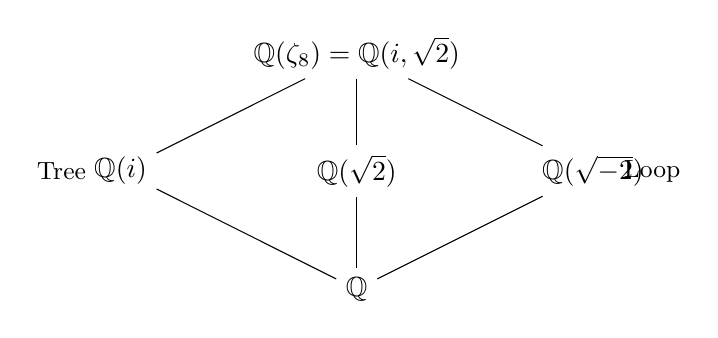
\begin{tikzpicture}[scale=1.5]
\node (top) at (0,2) {$\mathbb{Q}(\zeta_8) = \mathbb{Q}(i, \sqrt{2})$};
\node (left) at (-2,1) {$\mathbb{Q}(i)$};
\node (mid) at (0,1) {$\mathbb{Q}(\sqrt{2})$};
\node (right) at (2,1) {$\mathbb{Q}(\sqrt{-2})$};
\node (bottom) at (0,0) {$\mathbb{Q}$};

\draw (top) -- (left);
\draw (top) -- (mid);
\draw (top) -- (right);
\draw (left) -- (bottom);
\draw (mid) -- (bottom);
\draw (right) -- (bottom);

\node at (-2.5, 1) {\small Tree};
\node at (2.5, 1) {\small Loop};
\end{tikzpicture}
\end{center}

The loop character detects the squareclass $[-2]$, hence the associated Frobenius sign is $\chi_8^{-}(p)$.

\textbf{Physical Interpretation:} The Galois group $\text{Gal}(\mathbb{Q}(i)/\mathbb{Q})$ acts on CHY solutions by complex conjugation, suggesting a possible relation to parity/conjugation operations in four-dimensional kinematics.

%==========================================================================
\section{Conclusion}
%==========================================================================
We proved the $n=5$ splitting field statement and the loop square-class character, and computationally verified $n=7$ inert-prime vanishing and conjugate-pair structure on the fixed dataset $D_1$ under good reduction. A natural next computational step is to refine the block action $\overline{G}_7 \le S_{12}$ via cycle-type statistics over finite fields, and to extend verification to additional kinematic datasets.

%==========================================================================
\section*{Appendix: Reproducibility}
%==========================================================================

All computations are available at \url{https://github.com/zacharycraig1/arithmetic-chy-amplitudes.git}.

\textbf{Referee Quickstart:}
\begin{verbatim}
make docker-pull
make checksums
make verify-sage
make verify-math   # requires wolframscript
make verify-full   # full publication-grade verification
\end{verbatim}

\textbf{Key scripts:}
\begin{itemize}
\item \texttt{referee\_checks/verify\_n5\_discriminant.sage} --- n=5 squareclass verification
\item \texttt{referee\_checks/verify\_n7\_theorem.sage} --- n=7 inert vanishing
\item \path{referee_checks/verify_gram_levi.wl} --- Gram--Levi-Civita identity (Mathematica)
\item \texttt{referee\_checks/verify\_n7\_np2\_extension.sage} --- optional $\mathbb{F}_{p^2}$ extension check
\end{itemize}

%==========================================================================
\bibliographystyle{unsrt}
\begin{thebibliography}{99}

\bibitem{CHY2013}
F.~Cachazo, S.~He, and E.~Y.~Yuan,
``Scattering of Massless Particles in Arbitrary Dimensions,''
Phys.\ Rev.\ Lett.\ \textbf{113}, 171601 (2014),
arXiv:1307.2199 [hep-th].

\bibitem{CHY2014}
F.~Cachazo, S.~He, and E.~Y.~Yuan,
``Scattering Equations and Matrices: From Einstein To Yang-Mills, DBI and NLSM,''
JHEP \textbf{07}, 149 (2015),
arXiv:1412.3479 [hep-th].

\bibitem{CHYOrthogonality}
F.~Cachazo, S.~He, and E.~Y.~Yuan,
``Scattering equations and KLT orthogonality,''
Phys.\ Rev.\ D \textbf{90}, 065001 (2014),
arXiv:1306.6575 [hep-th].

\bibitem{Weinzierl2014}
S.~Weinzierl,
``On the solutions of the scattering equations,''
JHEP \textbf{04}, 092 (2014),
arXiv:1402.2516 [hep-th].

\bibitem{BDS}
Z.~Bern, L.~J.~Dixon, and V.~A.~Smirnov,
``Iteration of planar amplitudes in maximally supersymmetric Yang-Mills theory,''
Phys.\ Rev.\ D \textbf{72}, 085001 (2005),
arXiv:hep-th/0505205.

\bibitem{IrelandRosen}
K.~Ireland and M.~Rosen,
\emph{A Classical Introduction to Modern Number Theory},
Graduate Texts in Mathematics 84, Springer (1990).

\bibitem{CoxIVA}
D.~Cox, J.~Little, and D.~O'Shea,
\emph{Ideals, Varieties, and Algorithms},
4th ed., Springer (2015).

\bibitem{AdamsLoustaunau}
W.~W. Adams and P.~Loustaunau,
\emph{An Introduction to Gröbner Bases},
Graduate Studies in Mathematics 3, AMS (1994).

\bibitem{DixonMortimer}
J.~D. Dixon and B.~Mortimer,
\emph{Permutation Groups},
Graduate Texts in Mathematics 163, Springer (1996).

\end{thebibliography}

\end{document}
